\newcommand{\indentedlist}{\setlength\itemindent{0.5cm}}
\newcommand{\specialcell}[2][c]{\begin{tabular}[#1]{@{}c@{}}#2\end{tabular}}

Let $\beta$ be an arc belonging to a Burau pair $(\alpha, \beta)$ subject to the reductions of Section \ref{subsect:standardForms}. The boundary of a regular neighborhood of $\beta$ is a loop $\gamma$ supported on $\mu$, and thus we can get a set of weights for $\gamma$. In this section we go the opposite direction, finding necessary and sufficient conditions that a set of weights produces a multicurve $\gamma$, one component of which is a regular neighborhood of an arc $\beta$ belonging to a Burau pair $(\alpha, \beta)$ subject to the reductions of Section \ref{subsect:standardForms}. Not being able to give conditions on the weights to prevent proper multicurves from arising, we instead detect proper multicurves by performing a preliminary computation on a given weight set. Details on this as well as our algorithm are given at the end of this section.

\begin{figure}[h]
 \begin{center}
  \begin{overpic}[width=0.8\textwidth]{FSTrack.png}
   \put(0,1){$r_0$}
   \put(45,1){$r_1$}
   \put(78,1){$r_2$}
   \put(96,1){$r_3$}
   \put(8,13){$r_4$}
   \put(29,13){$r_5$}
   \put(61,13){$r_6$}
   \put(80,13){$r_7$}
   \put(27,19){$r_8$}
   \put(35,19){$r_9$}
   \put(30,24){$r_{10}$}
   \put(59,19){$r_{11}$}
   \put(67,19){$r_{12}$}
   \put(63,24){$r_{13}$}
   \put(45,24){$r_{14}$}
  \end{overpic}
  \caption{The train track $\mu$.}
  \label{fig:implementationTrainTrack}
 \end{center}
\end{figure}

With $\N$ the nonnegative integers, let $(w_i)_{i=0}^{14} \in \N^{15}$ where $w_i$ is the weight of the $i$th rail of $\mu$ as labeled in Figure \ref{fig:implementationTrainTrack}. The switch conditions are expressed by the following equations.
\begin{align*}
 w_4 &= 2w_0 & w_8 &= w_0 + w_1 - \frac{w_{14}}{2} & w_{11} &= w_2 - w_3 + \frac{w_{14}}{2}\\
 w_5 &= 2w_1 & w_9 &= -w_0 + w_1 + \frac{w_{14}}{2} & w_{12} &= w_2 + w_3 - \frac{w_{14}}{2}\\
 w_6 &= 2w_2 & w_{10} &= w_0 - w_1 + \frac{w_{14}}{2} & w_{13} &= -w_2 + w_3 + \frac{w_{14}}{2}\\
 w_7 &= 2w_3
\end{align*}
As every weight is freely determined by $w_0$, $w_1$, $w_2$, $w_3$, and $w_{14}$, 
we focus our attention on the tuple $(w_0, w_1, w_2, w_3, w_{14})$.

\textbf{Divisibility:} The arc $\beta$ starts on rail $6$ and ends on rail $7$, so weights $w_0$ and $w_1$ are even and weights $w_2$ and $w_3$ are odd. 
\begin{center}
 \begin{tabular}{clcclcclccl}
  D1. & $2 \mid w_0$ & \qquad \qquad & D2. & $2 \nmid w_1$ & \qquad \qquad & D3. & $2 \mid w_2$ && D4. & $2 \nmid w_3$
 \end{tabular}
\end{center}

\textbf{Nonnegativity:} The weights $w_8,\ w_9,\ w_{10},\ w_{11},\ w_{12},$ and $w_{13}$ must be nonnegative.
\begin{center}
 \begin{tabular}{clcclccl}
  N1. & $\frac{w_{14}}{2} \leq w_0 + w_1$ & \qquad \qquad & N3. & $w_1 \leq w_0 + \frac{w_{14}}{2}$ & \qquad \qquad & N5. & $\frac{w_{14}}{2} \leq w_2 + w_3$\\
  N2. & $w_0 \leq w_1 + \frac{w_{14}}{2}$ && N4. & $w_3 \leq w_2 + \frac{w_{14}}{2}$ && N6. & $w_2 \leq w_3 + \frac{w_{14}}{2}$
 \end{tabular}
\end{center}

In the next two groups of conditions, we ``steer'' the initial and terminal segments as dictated by the reductions in Section \ref{subsect:standardForms}. Consider the track segment seen in Figure \ref{fig:TrackSegment}. Which rail the arc follows is determined by the number of lines $\ell$ that are to the left of the arc as it approaches a switch. Beginning at the switch of $r_0$ and $r_1$ traveling left, $\ell = w_0$. The arc is steered left if and only if $w_0 < w_2$. Assuming this is the case, after passing through the switch of $r_2$ and $r_4$ we still have $\ell = w_0$. On the other hand if the arc is steered right, then after passing through the switch of $r_3$ and $r_4$ we now have $\ell = w_0 - w_2 + w_4$. As the notions ``initial'' and ``terminal'' are merely a choice of orientation, these remarks equally apply to the terminal segment of the arc.

\begin{figure}
 \centering
 \begin{subfigure}[t]{0.4\textwidth}
  \centering
  \begin{overpic}[scale=0.45]{TrainTrackSegment.png}
   \put(80,17){$r_0$}
   \put(42,26){$r_1$}
   \put(7,20){$r_2$}
   \put(7,42){$r_3$}
   \put(-8,32){$r_4$}
  \end{overpic}
  \caption{}
 \end{subfigure}
 \quad
 \begin{subfigure}[t]{0.4\textwidth}
  \centering
  \begin{overpic}[scale=0.45]{TrainTrackSegmentLeft.png}
   \put(80,10){$3$}
   \put(42,15){$6$}
   \put(14,14){$4$}
   \put(14,40){$2$}
   \put(2,30){$0$}
  \end{overpic}
  \caption{}
 \end{subfigure}
 \caption{A part of a train track where an arc is steered left.}
 \label{fig:TrackSegment}
\end{figure}


\textbf{Initial segment:} The arc $\beta$ starts on rail $6$ and then travels on rail $11$, meaning $w_2 < w_{11}$. After this, $\beta$ intersects the arc $\alpha$ from the top along rail $0$ or $1$, or from the bottom along rail $0$, meaning $w_9 < w_2$ or $w_1 < w_2$. In the case where $\beta$ intersects $\alpha$ from the bottom while traveling along rail $0$, we must enforce that $\beta$ does not then undo this intersection by traveling along rail $8$ and intersecting $\alpha$ from the top, as seen in Figure \ref{fig:badInitial}.

\begin{figure}[h]
 \begin{center}
  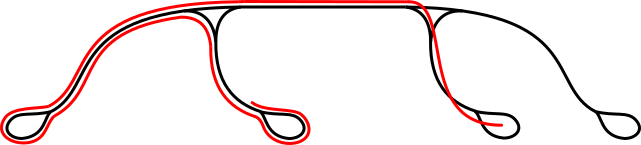
\includegraphics[scale=0.6]{FSTrack-HomotopedInitial.png}
  \caption{Initial intersection that can be homotoped off.}
  \label{fig:badInitial}
 \end{center}
\end{figure}

Therefore, if $w_9 < w_2$ and $w_0 < w_2 - w_9 + w_8$, then $w_2 - w_9 + w_8 < w_{10}$ or $w_2 + w_8 - w_{10} < w_1$. Using the switch conditions, we translate these into conditions on $w_0$, $w_1$, $w_2$, $w_3$, and $w_{14}$.
\begin{enumerate}[\indentedlist {I}1.]
 \indentedlist
 \item 
  $w_3 < \frac{w_{14}}{2}$
 \item
  $w_1 + \frac{w_{14}}{2}< w_0 + w_2$ \quad or \quad $w_1 < w_2$
 \item 
  $w_0 + w_2 < w_1 + \frac{w_{14}}{2}$ \quad or \quad $w_0 + w_2 < w_{14}$ 
\quad or \quad $w_0 + w_1 + w_2 < 3\frac{w_{14}}{2}$ \quad or \quad $w_1 + w_2 
< w_{14}$
\end{enumerate}

\textbf{Terminal segment:} The terminal segment of $\beta$ is seen in Figure \ref{fig:terminalPath}.
\begin{figure}
 \begin{center}
  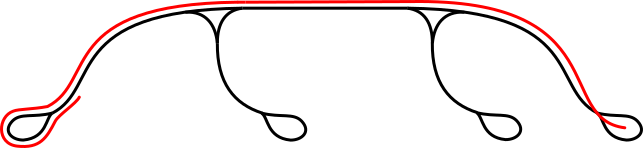
\includegraphics[scale=0.6]{FSTrack-Terminal.png}
  \caption{Terminal segment of an arc.}
  \label{fig:terminalPath}
 \end{center}
\end{figure}
This translates into the conditions $w_{12} < w_3$, $w_9 < w_3 - w_{12} + w_{11}$, and $w_0 < w_3 - w_{12} + w_{11} - w_9 + w_8$. Immediately prior to taking this path, the arc cannot travel on rail $1$ intersecting $\alpha$ from below. This gives the fourth condition
$$w_3 - w_{12} + w_{11} - w_9 + w_8 < w_{10} \quad \text{ or } \quad w_3 - 
w_{12} + w_{11} + w_8 - w_{10} < w_1.$$
Again using the switch conditions, we express these in terms of $w_0$, $w_1$, $w_2$, $w_3$, and $w_{14}$.
\begin{center}
 \begin{tabular}{clccl}
  T1. & $w_2 < \frac{w_{14}}{2}$ & \qquad \qquad & T3. & $w_3 < w_0$\\
  T2. & $w_1 + w_3 < w_0 + \frac{w_{14}}{2}$ && T4. & $w_0 + w_1 < w_3 + \frac{w_{14}}{2}$ \quad or \quad $w_1 < w_3$
 \end{tabular}
\end{center}

In order to prove that the conditions we have given are sufficient, we will use the following lemma.

\begin{lemma}[\cite{FM12}, Proposition 1.7]
 \label{lem:diagon}
 Two transverse simple closed curves $\alpha$ and $\beta$ in a surface $S$ cannot be homotoped to have fewer intersections if and only if they do not form a ``bigon'', that is, an embedded disk in $S$ whose boundary is the union of an arc of $\alpha$ and an arc of $\beta$.
\end{lemma}

\begin{proposition}
 \label{prop:sufficiency}
 The conditions D1-D4, N1-N6, I1-I3, and T1-T4 are necessary and sufficient for the weights $(w_i)_{i=0}^{14}$ to give rise to a multicurve $\gamma$, one component of which is a regular neighborhood of an arc $\beta$ belonging to a Burau pair $(\alpha, \beta)$ subject to the reductions of Section \ref{subsect:standardForms}.
\end{proposition}
\begin{proof}
 The necessity is clear. To show the sufficiency of the conditions, we must show that the initial and terminal intersections are essential. We prove a stronger statement, that the only nonessential intersection between $\alpha$ and $\beta$ supported on $\mu$ is of the form seen in Figure \ref{fig:badInitial}. Let $\alpha$ and $\beta$ intersect at $i_1$. Continuing to follow $\beta$, assuming it is not of the form in Figure \ref{fig:badInitial}, it must wind around a puncture $p_i$ before intersecting $\alpha$ again. Denote the next intersection of $\beta$ with $\alpha$ by $i_2$, and consider the loop $\eta$ formed by $\beta$ from $i_1$ to $i_2$ and $\alpha$ from $i_2$ to $i_1$. As $\eta$ is supported on the track, there is a corresponding set of weights $(v_i)_{i=0}^{14} \in \N^{15}$. The puncture $p_i$ will be interior to $\eta$ if and only if the corresponding weight $v_{i-1}$ is odd. If $v_0$, $v_1$, $v_2$, and $v_3$ are even, then by the switch conditions all the weights are even, implying that $\eta$ is a proper multicurve. Therefore one weight must be odd, so some $p_i$ is interior to $\eta$, and the result now follows from Lemma \ref{lem:diagon}.
\end{proof}

\begin{corollary}
 \label{cor:interesectionCount}
 Let $(w_i)_{i=0}^{14}$ be a set of weights as in Proposition \ref{prop:sufficiency} giving rise to a loop (and not a proper multicurve). Denote by $\beta$ the resulting arc. Then the number of essential intersections of $\alpha$ with $\beta$ is
  $$\frac{w_0}{2} + \frac{w_1}{2} - \min(w_1, w_8).$$
\end{corollary}

There are two ways we can prevent certain proper multicurves from arising. The first is to insist that $\gcd(w_0, w_1, w_2, w_3) = 1$, as otherwise all weights will share a non-trivial common factor and give rise to multiple copies of a single, simple closed curve. The second is to insist that some weight is zero, as otherwise the resulting multicurve will have a loop encompassing the entire train track and thus be a proper multicurve. The paths of the initial and terminal segments of the corresponding arc imply that all weights except for $w_1$, $w_8$, $w_9$, and $w_{12}$ are non-zero. Since $w_1$ being zero implies that $w_8$ and $w_9$ are zero, we have three cases.
\begin{enumerate}[(I)]
 \indentedlist
 \item
  $w_8 = 0$, meaning $\frac{w_{14}}{2} = w_0 + w_1$
 \item
  $w_9 = 0$, meaning $\frac{w_{14}}{2} = w_0 - w_1$
 \item
  $w_{12} = 0$, meaning $\frac{w_{14}}{2} = w_2 + w_3$
\end{enumerate}
All three cases can occur simultaneously. In each case, many of the above conditions become satisfied or simplified. The conditions D1-D4 remain in all cases, and the other conditions become the following.
\begin{center}
 Case I.
 
 N1. $w_0 + w_1 \leq w_2 + w_3$ \qquad I2. $w_1 < w_2$ \qquad T1. $w_2 < w_0 + w_1$ \qquad  T3. $w_3 < w_0$
\end{center}

\begin{center}
 Case II.
 
 \begin{tabular}{clccl}
  N5. & $w_0 \leq w_1 + w_2 + w_3$ & \qquad \qquad & I3. & $w_1 + w_3 < w_0$\\
  I1. & $w_0 < w_2 + 2w_1$ \quad or \quad $4w_1 + w_2 < 2w_0$  && T1. & $w_1 + w_2 < w_0$\\
  I2. & $w_1 < w_2$ && T4. & $w_1 < w_3$\\
 \end{tabular}
\end{center}

\begin{center}
 Case III.
 
 \begin{tabular}{clccl}
  N1. & $w_2 + w_3 \leq w_0 + w_1$ & \qquad & T2. & $w_1 < w_2 + w_0$\\
  N2. & $w_0 \leq w_1 + w_2 + w_3$ && T3. & $w_3 < w_0$\\
  I2. & $w_1 + w_3 < w_0$ \quad or \quad $w_1 < w_2$ && T4. & $w_0 + w_1 < w_2 + 2w_3$ \quad or \quad $w_1 < w_3$\\
  I3. & \multicolumn{4}{l}{$w_0 < w_1 + w_3$ \quad or \quad $w_2 + 2w_3 < w_0$ \quad or \quad $w_0 + w_1 < 2w_2 + 3w_3$}\\
 \end{tabular}
\end{center}

When traveling on rail $14$ either moving left or right, the conditions on the initial and terminal segments imply that there are only a finite number of possible paths one may take before returning to rail $14$. These paths are enumerated in Figure \ref{fig:paths}.
\begin{figure}
 \centering
 \begin{subfigure}{0.4\textwidth}
  \centering
  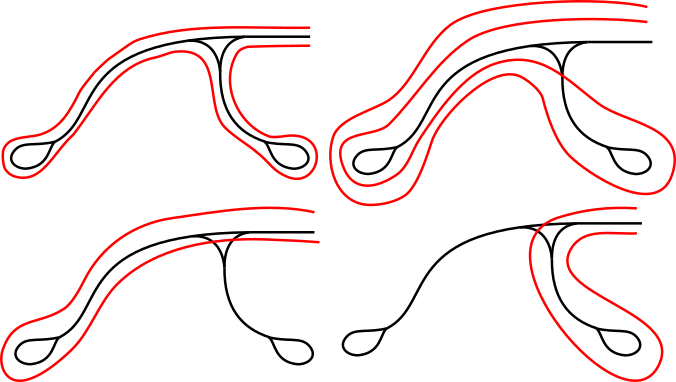
\includegraphics[scale=0.4]{LeftPaths.png}
  \captionof{figure}{Left paths.}
  \label{fig:leftPaths}
 \end{subfigure}
 \qquad \qquad
 \begin{subfigure}{0.4\textwidth}
  \centering
  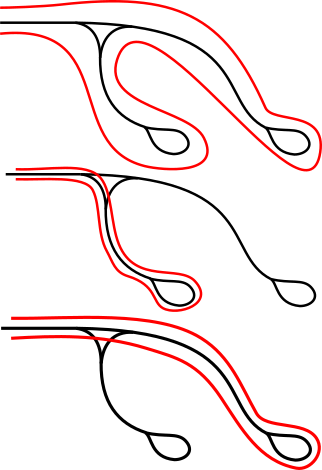
\includegraphics[scale=0.4]{RightPaths.png}
  \captionof{figure}{Right paths.}
  \label{fig:rightPaths}
 \end{subfigure}
 \caption{Enumeration of paths.}
 \label{fig:paths}
\end{figure}
Let $\ell$ denote the number of lines to the left of the arc as it travels on rail 14. Which of the enumerated paths is taken, along with the direction this path is traversed, is determined by comparing $\ell$ to the train track weights. When traveling to the left, the path and direction are determined by the position of the first number that $\ell$ is smaller than in the following list.
 $$\min(w_1, w_8, w_9),\ \min(w_1, w_9),\ w_9,\ w_0 + w_9 - w_8,\ w_{10} + w_9 - w_8,\ w_1 + w_{10} - w_8,$$
 $$w_{14} - w_1,\ \min(w_{10}, w_0 + w_{10} - w_8, 2w_{10} - w_8)$$
Likewise when traveling to the right, the path and direction are determined by the position of the first number that $\ell$ is smaller than in the following list.
 $$\min(w_3, w_{12}, w_{13}),\ \min(w_3, w_{13}),\ w_{13},\ w_2 + w_{13} - w_{12},\ w_{11} + w_{13} - w_{12}$$
Note that for a given set of weights, it may be that either of the lists are not ascending. This can occur when an arc never takes one of the paths enumerated in Figure \ref{fig:leftPaths} and Figure \ref{fig:rightPaths}. 

To compute the resulting Burau polynomial, our algorithm begins with $\ell = w_2$ and the Burau polynomial being $0$. We then alternate traveling left and right on rail $14$. Each time a path is taken, we update $\ell$ and the Burau polynomial accordingly. We end the computation when the arc reaches rail $7$ with $\ell = w_3$. While traveling right on rail 14, this is precisely when we have either $\ell = w_3$ and $\ell < \ w_{13}$, or $\ell$ is greater than all the numbers in the list above and $\ell = 3w_3 + w_{14}$. Along with being computationally efficient, this allows us to concisely describe the path of an arc. Each time we return to rail 14, using the appropriate list we record the position of the first number that $\ell$ is smaller than, $1-8$ and $1-6$ respectively. We call the resulting list \emph{the record of the arc $\beta$}.

We achieve a significant speedup by doing a preliminary run on each arc, recording the number of positive and negative crossings. We discard the weight set if a proper multicurve is ever detected, which by Corollary \ref{cor:interesectionCount} is the case if and only if the number of crossings is less than $\frac{w_0}{2} + \frac{w_1}{2} - \min(w_1, w_8)$. During the preliminary run, we also use a static array of size $2^m$ to compute the Burau polynomial where the powers of $t$ are treated modulo $2^m$. On our system, $m = 7$ appears to be optimal. When we are solely searching for the zero polynomial, we short-circuit the computation if the array is not all zero.
